% !TEX TS-program = latex
% !TEX root = Thesis_Guo2013.tex

\chapter{Introduction}
The tasks of estimation, inference and prediction, as an essential constituent of human activities, have been embraced by researchers in computer science, especially in the field of \textit{Artificial Intelligence (AI)}. 
To solve these tasks, researchers make use of both the mathematical formalism and the computational power realized by modern hardware and programming tools. 
Unfortunately, due to the continuing influences of the early pioneers and their paradigms, for a while AI scientists equated reasoning with ``rational'' deduction; and tried to come up with if-then-else rules for various prediction tasks \cite{ravikumar2007}.

However, in the recent several decades, a noticeable paradigm shift occurred in the field of AI. 
More modern influences such as quantum physics and statistics made many appreciate the use of probabilistic machinery, not just for modeling uncertainty but for making efficient estimations and predictions possible at all. From then on, scientists in AI growingly rely on probability theory and statistics as the formalism for seeking both theoretical insights into problems and justifications for methods and algorithms \cite{russell2010book}. 

Even a sub-field called \textit{machine learning} emerged from the general stream of AI. 
While AI emphasizes the study and design of intelligent agents, including  a group of interacting agents, as the central topic, machine learning is more specific in both its objective and methodology. Machine learning is concerned with discovering patterns, making inferences and predictions from \textit{data} and it shares the same formal framework with probability and statistics, which is also the paradigm adopted in this thesis.

In a probabilistic perspective, a central and fundamental task would be the characterization of the distribution of random variables, including the marginal of each variable and the interdependence among them. Ideally, the fullest characterization would be given by writing down the joint distribution of the all the variables involved. Yet, among others, due to the usually unknown or partially observable mechanism underlying real-world data or the ``curse of dimensionality'' coming with a large number of variables, one has to assume less accurate but more compact forms of representation of the joint distribution, such as log-linear models, Markov random fields and Bayesian networks \cite{bishop2006prml}.

Once we have data and the estimated distribution of the variables in concern, it would be desirable to know the properties of the distribution, for the purpose of developing learning algorithms that utilizes these properties or summarizing the large-volume data into a straightforward, human-perceptible form. Among others, moments are the simplest measures for quantitatively characterizing the shape of distributions. For example, if we have the data tracking a noisy signal and find that the signal follows a Gaussian distribution, we would then like to know the mean and standard deviation of the noise, for the first measure tells us around what value the signal fluctuates and the second informs us the amplitude of the fluctuation. 

Moments are also important in their role connecting data and the population. In a statistical point of view, the data collected are considered as a part out of an infinite sea of data that are not fully observed, which are called \textit{statistical population}. On one hand, we use the data to estimate the distribution of population; on the other hand, we assume that future, unobserved data and the data available now are sampled from \textit{the same} population so that our model can be \textit{generalized} to unknown or future cases. 

Specifically, a moment simultaneously corresponds to a sample moment and a population moment, where the former characterizes how data in hands are distributed and the latter characterizes how the population are distributed. A sample moment is computed by performing simple algebraic operations on data, e.g. the arithmetic mean is the sum of all observation of a variable divided by the number of observations; a population moment is obtained by getting the mathematical expectation of a polynomial function of the random variable, which is usually done in the form of integral, e.g. the population mean is the mathematical expectation of the random variable itself.  

The relation between the sample moments and the corresponding population moments are known when the population moments converge --- a sample moment converges to the corresponding population moment by probability when the size of samples extends to infinity. Therefore, in the convergent case, we can use the sample moments calculated with a large sample to estimate the shape of the population distribution. In the traditional statistical literature, because the distributions encountered (e.g. Gaussian, exponential) are usually exponentially bounded in tails, population moments of all positive orders would naturally converge. As a result, the convergence of moments are often assumed without explicit mention and the relation between the two kinds moments is largely ``taken for granted'' in practice.

However, such a naive notion towards moments and the general assumption of moments being convergent should be brought to serious examination when dealing with today's ever diversified data. A distinctive exception to the moment-convergent assumption is a family of distributions called \textit{heavy-dutyed distributions}, where the density functions in this family have heavier tails than the exponential distributions \cite{asmussen2003applied}, rendering their moments with orders higher than a threshold divergent. Heavy-tailed distributions ``appear'' more common than before with the development of information technology, as data can now be collected and assembled from an unprecedented large scale, e.g. data collected from the whole Internet, from millions of online users and from hundreds of countries around the world. For example, \textit{power-law distributions}, as a member of the heavy-tail family, are found in the distributions for the degrees of the Internet, the population of cities around the world and the citations of papers in academic communities \cite{Clauset2009}. 

When dealing with data exhibiting these distributions, it is possible that a certain moment of interest is divergent. Then, the sample moment do not converge when the sample size grows bigger, but instead grows with the size. In this thesis, I will first seek to clarify the underlying mechanism beneath the divergence of moments and the relation between sample and population moments in this case. Then I will propose a method that systematically analyzes the asymptotic behavior of sample moments under convergence as the sample size extends to infinity. Furthermore, I will discuss the application of this method in analyzing heavy-tailed distributions, especially power-law distributions. Before addressing the method for analyzing divergent moments, I would like to outline some key concepts involved as background materials for this work.

\section{Random variables and probability distributions}
\subsection{Random variables}
Probability theory deals with the analysis of the likelihood of random events defined over a sample space $ \Omega $ . For example, consider rolling a single fair die, where we denote the value rolled as $ X $ and the sample space as $ \Omega $. The sample space of a single roll can be defined as $\Omega = \{1, 2, 3, 4, 5, 6\}$ and the possible random events are subsets of $ \Omega $ . For example, we can consider the event that $ X=4 $  is rolled as well as the event that an even value is rolled. If an event is a single element of the sample space $ X \in \Omega $  then we refer to the event as an atomic event. The event that $ X=4 $  is rolled is an example of an atomic event.

When dealing with random events we are often interested in numerical descriptions of the events and not just the probability of the event occurring. In order to handle this we can assign numerical descriptions of events to what are referred to as random variables. For example, $ X $ is a random variable in rolling one fair die. And supposing that we roll two fair dice, we also can define a random variable $ Y $  to take on the numerical result of the sum of the dice. 

\begin{defn}
A random variable $ X $  defined over a sample space $ \Omega $  is a function $ X: \Omega \rightarrow \mathbb{R} $ that maps an event $ X \in \Omega $  to a real value.
\end{defn}

Random variables that only take on values from a countable set (such as the integers) are referred to as discrete random variables. The random variable defined as the sum of the roll of two fair dice is an example. Random variables that take on values from an uncountable set (such as the reals) are referred to as continuous random variables. For example, the arrival time for the next car in a highway intersection is a continuous random variable.

\subsection{Probability distributions}
In analyzing random variables we are often interested in the probability that a random variable takes on certain values. To formally describe the different probabilities of a random variable taking on various values we define a probability distribution.

\begin{defn}
A probability distribution $ P $ defined on random variable $ X $  over a sample space $ \Omega $  is a mapping from events $ \alpha \in \Omega $  to real values on the interval $ [0,1] $  such that $ P(\alpha) \geq 0 $  and $ P(\Omega)=1 $ .
\end{defn}


\section{Moment}
In statistics, a moment is, loosely speaking, a quantitative measure of the shape of a distribution. For example, mean, as the simplest moment, measures around what value the distribution is centered around; and variance, as the second central moment, measures how much the distribution disperses around the mean; while some moments of higher orders describe other aspects of a distribution such as how the distribution is skewed from its mean, or peaked. While moments can be extended to multivariate distributions, such as \textit{image moments} that are used in 2-D image processing \cite{hu1962visual}, we will focus on univariate distributions due to the scope of this thesis. 

\subsection{Expectation and Riemann-Stieltjes integral}
A population moment with regard to a probability distribution is formally defined as the \textit{mathematical expectation} of a polynomial function of the random variable. And a rigorous, unified treatment of expectation relies \textit{Riemann-Stieltjes integral}, which is a generalized form for the \textit{Riemann integral}. Therefore, we will first briefly outline these concepts before moments are introduced.

Whereas the usual Riemann integral of a real-valued function $ g(x) $ with regard to the variable $ x $ on a range $ [a,b] $ is usually denoted by $ \int_a^b g(x) dx $, a Riemann-Stieltjes integral for $ x $  involves two functions. The Riemann-Stieltjes integral for $ g(x) $ with regard to another real function $ F(x) $ is denoted by $ \int_a^b g(x)dF(x) $. It is well-known that $ \int_a^b g(x) dx $ can be interpreted as the area under $ g(x) $ with $ a \leq x \leq b $. So what does Riemann-Stieltjes integral mean? In fact, $ \int_a^b g(t) dF(t) $ (the variable is changed for convenience) can still interpreted as the area under a curve. Let us imagine $ t $ as a parameter and we now track the point $ t $ moving from $ a $ to $ b $, meanwhile drawing the curve $ (x,y)=(F(t), g(t)) $. Then the integral is simply the area under the curve, as a sum of rectangles each resulted by a every tiny move of $ t $. 

Now let us turn to a more formal definition of $ \int_a^b g(x)dF(x) $. First the range $ [a,b] $ is partitioned into $ n $ intervals with  $ a=x_0 < x_1 < \cdots < x_{n-1} < x_n=b$. Then we tag each small interval $ [x_i, x_{i+1}] $ with a representative number $ c_i $, with $ c_i \in [x_i, x_{i+1}] $. Next, 
we write down the sum of the area of small rectangles as 
\begin{equation}
S = \sum_{i=0}^{n-1} g(c_i) (F(x_{i+1})-F(x_i)).
\end{equation}
The integral can obtained by taking the limit of $ S $ while ``densifying'' the partition. The density can be measured by a \textit{mesh} of the partition, and here we just take the maximum length of the interval $ \Delta = \max_{0 \leq i \leq n-1} (x_{i+1}-x_{i})$ as the mesh. As the mesh $ \Delta \rightarrow 0 $, the partition is continually densified and the sum would converge to a limit, if it exists, which is defined to be the Riemann-Stieltjes integral. Hence, we outline the following definition. 

\begin{defn}
If there is some $ A \in \mathbb{R} $, such that for any $ \epsilon > 0 $, there exists $ \delta > 0 $ so that any $ S = \sum_{i=0}^{n-1} g(c_i) (F(x_{i+1})-F(x_i)) $ with the mesh of partition $ \Delta < \delta  $ satisfies $ |S-A|< \epsilon $, then the Riemann-Stieltjes integral $ \int_a^b g(x) dF(x) $ exists and we define $ \int_a^b g(x) dF(x) \triangleq A $.  
\end{defn}

Now we turn to the definition for mathematical expectation. For a discrete random variable $ X $, which takes values $ x_1, x_2, \cdots, x_n $ with probabilities $ p_1, p_2, \cdots, p_m $, then the expectation of $ X $ is defend to be the weighted sum, i.e.
\begin{equation}
\E[X] = \sum_{i=1}^n x_i p_i. 
\end{equation}
For a continuous random variable $ X $ with a well-defined PDF $ f(x) $, then the expectation is yield with a Riemann integral, i.e.
\begin{equation}
\E[X] = \int_{-\infty}^{+\infty} x f(x) dx.
\end{equation}
It seems that expectation needs to be treated differently for discrete and continuous variables when the Riemann-Stieltjes integral comes to the rescue. 

\begin{defn}
Given $ X $ is a random variable with its cumulative distribution function (CDF) $ F(X) $, then its expectation value is defined to be 
\begin{equation}
\E[X] = \int_{-\infty}^{+\infty} x dF(x),
\end{equation}
regardless of $ X $ being discrete or continuous. 
\end{defn}
Similarly, the expectation of the random variable $ g(X) $ as a function of $ X $ is given by
\begin{equation}
\E [g(X)] = \int_{-\infty}^{+\infty} g(x) dF(x).
\end{equation}

\subsection{Definition of moment}
Every moment is defined with its ``double identity'' --- a population moment and sample moment. Both of them are quantitative measures for the shape of the distributions, but the former is for describing the shape of the ``empirical distribution'' (the distribution for samples), i.e. the CDF constructed from data, while the latter is for characterizing the distribution of population, where a well-defined, closed-form distribution function is usually assumed. When the sample size is small, the two distributions may be different and the two moments may also differ noticeably in their values; but when the sample size grows big, the empirical distribution  will converge to that of the population by the \textit{Strong Law of Large Numbers}, and the two moments will be identical in the limit. 

But the sample moment and its corresponding population moment are different in their calculation. Without explicitly getting the CDF for the empirical distribution, one can directly calculate sample moments by performing simple algebraic operations (addition, multiplication and division) on data. But the calculation of population moment is analytic, rather than algebraic. The population distribution is usually given (or assumed to be) as a analytic function and its population moments, if exist, can be acquired by integrating a polynomial function with regard to the PDF. These two moments are also different in their existence: a population moment does not exist if the integral diverges; a sample moment $ always $ exists because it is a algebraic outcome computed from data.

\subsubsection{Population moment}
A \textit{population moment} can be understood as a particular distance measure defined by the distribution with a point as its reference. When there is no ambiguity, we also refer to \textit{population moment} as \textit{moment} for short. 
\begin{defn}
Given a univariate PDF $ f(x) $ for the distribution of a random variable $ X $ , the $ n $-th moment taken about a point $ c $ is defined as $ \mu_n(c) = \int_{-\infty}^{+\infty} (x-c)^n f(x) dx $ \footnote{When addressing the definition of moments, we assume $ X $ is a continuous variable for simplicity. The discrete case can be similarly defined by replacing the integral with sum.} , if the integral converges.   
\end{defn}

The reference point $ c $ is often chosen to be $ 0 $ or the mean. When $ c=0 $, the moment is called \textit{raw moment}.

\begin{defn}
The $ n $-th raw moment is defined as $ \mu'_n = \mu_n(0) $, where $ \mu_n(c) $ is the moment taken about $ c $. 
\end{defn}
    
$ \mu'_1 $ is simply the $ mean $ of the distribution, and we have $ \mu'_0=1 $ due to the normalization of a distribution. For moments of higher orders, we are often concerned with the moment taken around the mean, which is called \textit{central moment}.

\begin{defn}
The $ n $-th central moment is defined as $ \mu_n = \mu_n(\mu'_1) $, where $ \mu_n(c) $ is the moment taken about $ c $ and $ \mu'_1 $ is the mean.    
\end{defn}

It shall be noted the following definitions rely on the condition that the integral for defining the moment is convergent, which is always the case for distributions with exponentially bounded tails, but not necessarily true for other distributions. 

\subsubsection{Sample moment}
\textit{Sample moments} are the same metrics as population moments, except that they are defined by the \textit{empirical distributions} of data, rather than the assumed the distribution function. Sample moments can be computed by performing simple algebraic operations on data and every moment $ \mu_n(c) $ has one sample counterpart $ m_n(c) $.

\begin{defn}
Given a sample $ \{x_1, x_2, \cdots, x_N\} $ with size $ N $, the $ n $-th sample moment with reference to $ c $ is defined as $ m_n(c) = \frac{1}{N} \sum_{i=1}^N (x_i-c)^n $.
\end{defn}

As samples are always finite numbers, a sample moment \textit{always} exists regardless of existence of the corresponding population moment. \textit{Sample raw moments} can be defined in a parallel fashion.

\begin{defn}
Given a sample $ \{x_1, x_2, \cdots, x_N\} $ with size $ N $, the $ n $-th sample raw moment is defined as $ m'_n = m_n(0) $.  
\end{defn}

Sample moments can be used as estimators for the corresponding population moments, which we would discuss later.

\subsection{Moments in common uses}
We now describe some population moments that are widely used in statistics for characterizing the shape of distributions. 

\subsubsection{Mean}
Mean is the first raw moment $ \mu'_1 $, which gives the value around which the distribution is centralized around.

\begin{figure}[!h]
\begin{center}
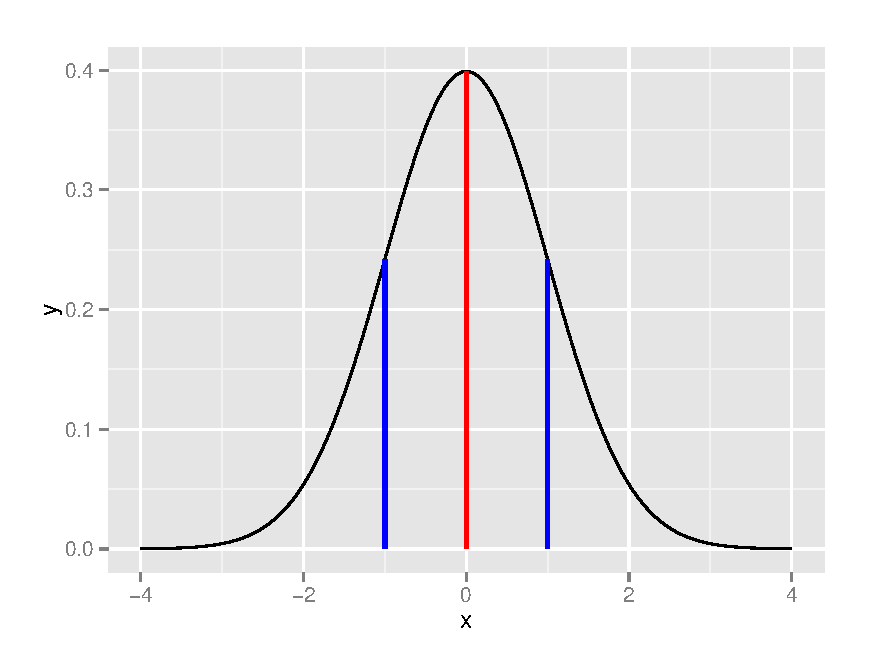
\includegraphics[width=0.8\textwidth]{figures/ch1_gaussian.eps}
\caption{The PDF for a standard Gaussian distribution, where the red vertical marks the value of $ \mu_1' $ and two blue lines mark $ \pm \sigma$. }
\label{fig:ch1_meanvar}
\end{center}
\end{figure}

\subsubsection{Variance}
Variance is the second central moment $ \mu_2 $, which describes how far the distribution spreads out around the mean. Its positive squared root $ \sigma $ is referred to as the \textit{standard deviation}. For the special case of Gaussian distributions, the distribution can be fully characterized by the mean and the variance, as shown in Fig. \ref{fig:ch1_meanvar}.

\subsubsection{Skewness}
The third central moment $ \mu_3 $ is a measure of the lopsidedness of the distribution; any \textit{symmetric} distribution will have a third central moment, if defined, of zero. When using higher order moments, it is a common practice to normalize the $ k $-th moment by the standard deviation to the power of $ k $.  

\begin{defn}
The $ k $-th standardized moment for a probability distribution is defined as $ \mu_k / \sigma^k $, where $ \mu_k $ is the $ k $-th central moment and $ \sigma $ is the standard deviation.
\end{defn}

In other words, the $ k $-th standardized moment is simply a \textit{normalzied} version of the $ k $-th moment with respect to the standard deviation. The power of $ k $ is used, because moments scale as $ x^k $ , meaning that $ \mu_k'(\lambda X) = \lambda^k \mu_k'(X) $:  they are homogeneous polynomials of degree $ k $ , thus the standardized moment is \textit{scale invariant}. This can also be understood as being because moments have dimension; in the above ratio defining standardized moments, the dimensions cancel, so they are dimensionless numbers.

Specifically, the \textit{standardized} third central moment $ \mu_3 / \sigma^3 $ is called the skewness, often denoted by $ \gamma_1 $, i.e.

\begin{defn}
The skewness for a random variable $ X $ is defined as $ \gamma_1 = \E[(\frac{x-\mu}{\sigma})^3] = \frac{\mu_3}{\sigma^3} $, where $ \mu $  
\end{defn}

As plotted by Fig. \ref{fig:ch1_skew}, a distribution that is skewed to the left (the tail of the distribution is heavier on the left) will have a negative skewness. A distribution that is skewed to the right (the tail of the distribution is heavier on the right), will have a positive skewness.

\begin{figure}[htbp]
\begin{center}
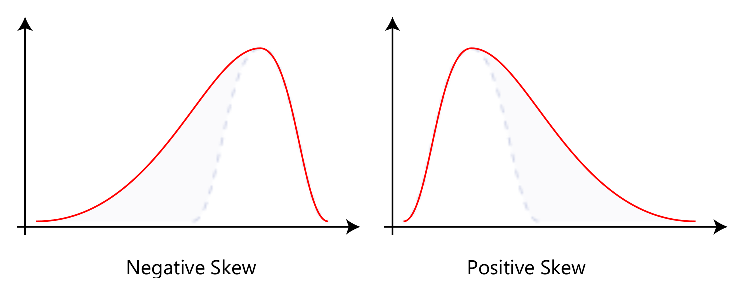
\includegraphics[width=0.8\textwidth]{figures/ch1_skew.eps}
\caption{Probabilty distributions with a negative skewness has a fatter or longer tail on the left side, and distributions with a positive skewness has a fatter or longer tail on the right side. (figure excerpted from \cite{www-wiki-skewness})}
\label{fig:ch1_skew}
\end{center}
\end{figure}

\subsubsection{Kurtosis}
The fourth central moment is a measure of whether the distribution is tall and skinny or short and squat, compared to the normal distribution of the same variance. Since it is the expectation of a fourth power, the fourth central moment, where defined, is always non-negative. 

One common measure of kurtosis, originating with Karl Pearson, is based on a scaled version of the fourth moment of the data or population, but it has been argued that this measure really measures heavy tails, and not peakedness. It is common practice to use an adjusted version of Pearson's kurtosis, the excess kurtosis, to provide a comparison of the shape of a given distribution to that of the normal distribution ($ \mu_4 $ for a normal distribution is $ 3\sigma^4 $). Fig. \ref{fig:ch1_kurtosis} shows three distributions of the same family with different values of kurtosis. 

\begin{defn}
The excess kurtosis for a random variable, if it exists, is defined as $ \gamma_2 = \mu_4 / \sigma^4 -3 $, where $ \mu_4 $ is the fourth central moment and $ \sigma $ is the standard deviation.
\end{defn}

\begin{figure}[!h]
\begin{center}
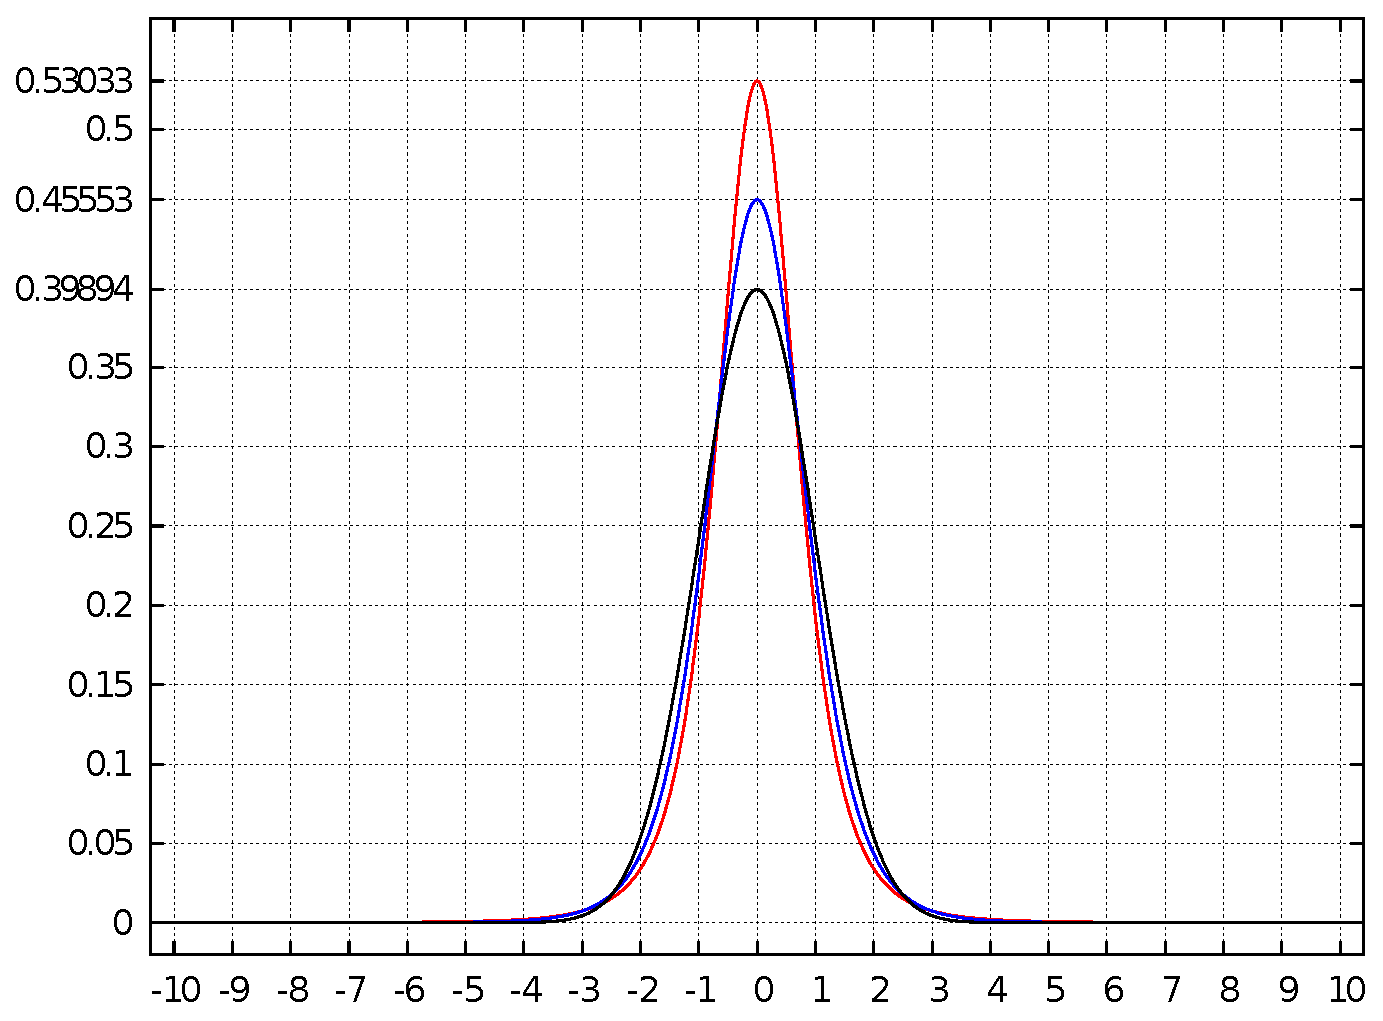
\includegraphics[width=0.7\textwidth]{figures/ch1_kurtosis.eps}
\caption{PDF for the Pearson type VII distributions with kurtosis of infinity (red), 2 (blue) and 0 (black). }
\label{fig:ch1_kurtosis}
\end{center}
\end{figure}

\subsubsection{Covariance and correlation coefficient}
\textit{Covariance} and \textit{correlation} are \textit{mixed moments} of most frequent uses. While the aforementioned moments only involve a single random variable, \textit{mixed moments} are moments of multiple random variables. 

In probability theory and statistics, covariance is a measure of how much two random variables change together. If the greater values of one variable mainly correspond with the greater values of the other variable, and the same holds for the smaller values, i.e., the variables tend to show similar behavior, the covariance is positive. In the opposite case, when the greater values of one variable mainly correspond to the smaller values of the other, i.e., the variables tend to show opposite behavior, the covariance is negative. The sign of the covariance therefore shows the tendency in the linear relationship between the variables.

\begin{defn}
The covariance between two jointly distributed real-valued random variables $ X $  and $ Y $  with finite second moments is defined as
\begin{equation}
\sigma(x,y) = \E \left [ (X-\E(X))(Y-E(Y)) \right].
\end{equation}
\end{defn}

After some algebra, covariance can be rewritten in the form as 
\begin{align}
\sigma(X,Y)
&= \operatorname{E}\left[\left(X - \operatorname{E}\left[X\right]\right) \left(Y - \operatorname{E}\left[Y\right]\right)\right] \nonumber\\
&= \operatorname{E}\left[X Y - X \operatorname{E}\left[Y\right] - \operatorname{E}\left[X\right] Y + \operatorname{E}\left[X\right] \operatorname{E}\left[Y\right]\right] \nonumber \\
&= \operatorname{E}\left[X Y\right] - \operatorname{E}\left[X\right] \operatorname{E}\left[Y\right] - \operatorname{E}\left[X\right] \operatorname{E}\left[Y\right] + \operatorname{E}\left[X\right] \operatorname{E}\left[Y\right] \nonumber \\
&= \operatorname{E}\left[X Y\right] - \operatorname{E}\left[X\right] \operatorname{E}\left[Y\right].
\end{align}

The definition above can also be extended to the case of more than two random variables, where covariance is formed as a matrix.
\begin{defn}
Supposing $ \bm{X} $ and $ \bm{Y} $ are two random vectors of dimension $ m $ and $ n $ respectively, each with finite second moment, then $ m \times n $ \textit{covariance matrix} is defined as 
\begin{align}
\bm{\sigma}(\bm{X}, \bm{Y}) &= \E \left [ (\bm{X} - \E(\bm{X}))(\bm{Y} - \E (\bm{Y}))^T \right ] \\
&= \E \left [ \bm{X} \bm{Y}^T \right ] - E[\bm{X}]E[\bm{Y}]^T.
\end{align}
\end{defn}

Whereas one can learn the consistency between two random variables (or two random vectors) from the sign of covariance, the value itself is often hard to interpret. Therefore, its standardized version, the \textit{correlation coefficient} is introduced as a measure lying in $ [-1,+1] $ to show the strength of linear relation.

In statistics, the \textit{Pearson product-moment correlation coefficient} (sometimes referred to as PCC, Pearson's $ r $, or correlation coefficient) is a measure of the \textit{linear correlation} (dependence) between two variables $ X $  and $ Y $ , giving a value between $ -1 $ and  $ +1 $ inclusive. It is widely used in the sciences as a measure of the strength of linear dependence between two variables.

Pearson's correlation coefficient between two variables is defined as the covariance of the two variables normalized by the product of their standard deviations. The form of the definition involves a ``product moment'', that is, the mean (the first moment about the origin) of the product of the mean-adjusted random variables.

\begin{defn}
The correlation coefficient $ \rho_{X,Y} $ for two random variables $ X $ and $ Y $, each with finite second moment, is defined as 
\begin{equation}
\rho_{X,Y} = \frac{\sigma(X,Y)}{\sigma_X \sigma_Y} = \frac{\E\left [ (X-\E[{X}])(Y-\E[{Y}])  \right ]}{\sigma_X \sigma_Y}.
\end{equation}
\end{defn}

The correlation coefficient can also be viewed as the product of the two \textit{standardized} random variables, i.e.
\begin{equation}
\rho_{X,Y} = \E \left [ \left ( \frac{X-\E(X)}{\sigma_X} \right ) \left ( \frac{Y-\E (Y)}{\sigma_Y} \right ) \right ].
\end{equation}
By regarding the expectation of the product of two variables as an \textit{inner product} between the two, i.e. $ \langle X,Y \rangle \stackrel{\Delta}{=} \E(XY)$, then due to the famous \textit{Cauchy-Schwartz inequality}, we have
\begin{align}
\rho_{X,Y}^2 & = \langle \frac{X-\E (X)}{\sigma_X}, \frac{Y - \E(Y)}{\sigma_Y} \rangle^2 \nonumber \\
& \leq \frac{\langle X - \E (X), X-\E (X) \rangle}{\sigma_X^2} \frac{\langle Y - \E (Y), Y-\E (Y) \rangle}{\sigma_Y^2} = 1,
\end{align}
from which we see that $ \rho $ is naturally bounded inside $ [-1,+1] $. And there is another advantage to standardize the covariant --- to make correlation coefficient a \textit{scale invariant} measure such that any \textit{linear transform} applied to one variable does not affect the outcome.
%TODO% mention bounds for pl

By replacing the population moments with the corresponding sample moments, we can write down the correlation coefficient for two samples $ (x_1, x_2, \cdots, x_n) $ and $ (y_1, y_2, \cdots, y_n) $ as 
\begin{equation}
\rho_{x,y} = \frac{\sum_{i=1}^{n} (x_i - \overline{x})(y_i - \overline{y})}{\sqrt{\sum_{i=1}^n(x_i-\overline{x})^2} \sqrt{\sum_{i=1}^n (y_i - \overline{y})^2} }.
\end{equation}
$ \rho_{x,y} $ is usually computed from data to reflect the linear relation between two variables of observation, which could be interpreted as the the cosine of the angle between both possible regression lines $ y=g_x(x) $  and $ x=g_y(y) $ geometrically. Fig. \ref{fig:ch1_corr_ex} plots several sets of points and their corresponding values of correlation coefficient. It shall be noted that the correlation coefficient only reflects the \textit{strength} of the linear relation, not to be confused with the \textit{slope} of linearity.

\begin{figure}[htbp]
\begin{center}
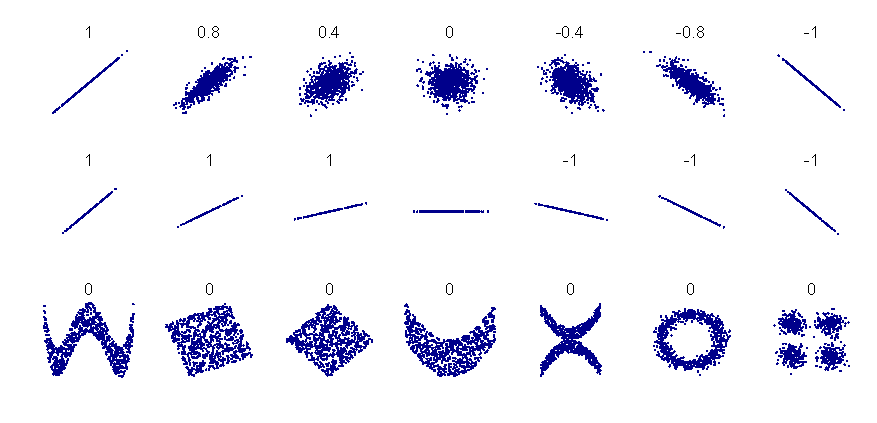
\includegraphics[width=0.8\textwidth]{figures/ch1_correlation.eps}
\caption{Several sets of $ (x,y) $  points, with the correlation coefficient of $ x $  and $ y $  for each set. Note that the correlation reflects the non-linearity and direction of a linear relationship (top row), but not the slope of that relationship (middle), nor many aspects of nonlinear relationships (bottom). (figure excerpted from \cite{www-wiki-corr})}
\label{fig:ch1_corr_ex}
\end{center}
\end{figure}


\subsection{Properties}


\subsubsection{The relation between raw moment and central moment}
The central moments $ \mu_n $  can be expressed as terms of the raw moments $ \mu_n' $ (i.e. those taken about zero) using the binomial transform \cite{papoulis2002probability}. 

\begin{thm}
The $ n $-th population central moment $ \mu_n $ can be expressed as 
\[ \mu_n = \sum_{k=0}^n \tbinom nk (-1)^{n-k} \mu_k' \mu_1'^{n-k}, \]
where $ \mu_k' $ is the $ k $-th raw moment. 
\end{thm}

\subsubsection{Moment-generating function}
Population moments, if exist, can also be obtained with \textit{moment-generating functions}. 

\begin{defn}
The moment-generating function for a random variable $ X $ is defined as 
\[ M_X(t) = \E[e^{tX}],\quad t \in \mathbb{R}, \]
whenever the expectation exists.
\end{defn}

The moments inside the function can be seen via the Taylor expansion as 
\begin{align*}
M_X(t) = \E[e^{tX}] &= \E \left [ 1+tX+\frac{(tX)^2}{2!} + \frac{(tX)^3}{3!} + \cdots \right ] \\
&= 1+ t\mu_1' + \frac{t^2}{2!} \mu_2' + \frac{t^3}{3!} \mu_3' + \cdots .
\end{align*}
By taking the $ n $-th order derivative and setting $ t=0 $, the term with $ \mu_n' $  with be left out while other terms vanish. Therefore, we have
\begin{equation}
\mu_n' = \E[X^n] = \frac{d^n M_X(0)}{dt^n}.
\end{equation}





